% NCD-CIE v29 — Minor revision addressing final panel feedback
%   - Highlighted FOURIER/EMPA-REG independent holdout in abstract + contributions
%   - Converted γ sensitivity to compact table with HTE ranking stability
%   - Strengthened Holm-Bonferroni and Hosmer-Lemeshow visibility
%   - Added QRISK3 to NNT/C-for-benefit comparison
% NCD-CIE v28 — Reviewer response revision (14-page LNCS limit)
%   - R1.1: Expanded cycle handling with temporal ordering + Tarjan + verification
%   - R1.2: Added attenuation sensitivity analysis paragraph
%   - R1.3: Added E-value table with interpretation
%   - R1.4: Added runtime note to Table 1
%   - R2.1: Added benefit-based vs risk-based comparison (NNT, C-for-benefit)
%   - R2.2: Added age-stratified AUC table with recalibration roadmap
%   - R2.3: Expanded NL parser evaluation (5 categories, failure modes)
%   - R2.4: Added clinical workflow description
%   - R3.1: Softened ρ=0.89 language (abstract, contributions, eval, conclusion) + bootstrap CI
%   - R3.2: Confirmed Holm-Bonferroni correction on all pairwise tests
%   - R3.3: Added Hosmer-Lemeshow calibration assessment for SCORE2
%   - R3.4: Clarified ablation design as independent component removal
% NCD-CIE v27 — Page-count reduction for LNCS (target ≤16 pages)
%   - Compressed causal forest literature review
%   - Merged HTE subsections, Risk Engine subsections
%   - Removed redundant figures (4, 5, 6) and Table 2
%   - Merged Implementation + Safety sections
%   - Moved full edge specification to supplementary only
%   - Tightened Discussion, removed redundancy
%   - Verified rung-3 language consistency
%   - Moved NL parser evaluation into LLM section
% v26: Added quantitative NL parser evaluation, addressed age >60 AUC drop
% v25: Added publication-quality visualizations
\documentclass[runningheads]{llncs}
\usepackage[T1]{fontenc}
\usepackage{graphicx}
\graphicspath{{figures/}}
\usepackage{amsmath,amssymb}
\usepackage{booktabs}
\usepackage{hyperref}
\usepackage{url}
\usepackage{multirow}
\usepackage{xcolor}

% Space-saving for page limit
\setlength{\textfloatsep}{4pt plus 1pt minus 2pt}
\setlength{\floatsep}{4pt plus 1pt minus 2pt}
\setlength{\intextsep}{4pt plus 1pt minus 2pt}
\setlength{\abovecaptionskip}{3pt}
\setlength{\belowcaptionskip}{1pt}
\setlength{\abovedisplayskip}{4pt}
\setlength{\belowdisplayskip}{4pt}
\setlength{\parskip}{0pt plus 0.5pt}

\titlerunning{NCD-CIE: Causal-Informed Clinical Decision Support}

\begin{document}

\title{NCD-CIE: A Causal-Informed Clinical Decision Support\\System with LLM Augmentation for\\Non-Communicable Disease Healthcare}

\author{Anonymous Submission}
\authorrunning{Anonymous}
\institute{Anonymous Institution}

\maketitle

%--------------------------------------------------------------
\begin{abstract}
Non-communicable diseases account for over 74\% of global mortality,
yet existing risk calculators cannot answer what-if questions about
interventions or identify \emph{which patients benefit most} from
treatment.
We present \textbf{NCD-CIE}, an open-source causal-informed clinical
decision support system with three core components augmented by large
language model (LLM) integration:
(i)~an expert-curated causal knowledge graph with 107 directed edges
across 8 clinical domains,
(ii)~a logistic-link risk engine with uncertainty quantification, and
(iii)~a topological what-if simulator enabling heterogeneous treatment
effect (HTE) estimation to identify high-benefit patients.
Three LLM augmentation layers extend clinical accessibility:
graph validation achieving 87.9\% expert agreement,
natural language query parsing (92\% accuracy), and
counterfactual explanation generation.
Outcome-based validation on the Framingham Heart Study cohort
($n\!=\!4{,}172$; 10-year follow-up) using \emph{independent} SCORE2
coefficients yields AUC-ROC\,=\,0.704---a deliberate tradeoff
favoring interpretability and HTE estimation over discriminative
performance.
Empirical HTE validation against SPRINT and FOURIER trial subgroup
analyses shows Spearman $\rho = 0.89$ (95\% CI: 0.55--0.97;
bootstrap: 0.52--0.96)
between predicted individual treatment effects and observed hazard
ratios across 10 patient subgroups, with \emph{independent holdout}
trials (FOURIER, EMPA-REG) reserved from parameter tuning,
providing preliminary evidence
that NCD-CIE can identify high-benefit patients.
Current validation focuses on primary prevention in adults 30--60;
performance declines in elderly populations (AUC\,=\,0.591 for
$>$60\,years), warranting age-specific recalibration.

\keywords{Causal knowledge graph \and Clinical decision support \and
Heterogeneous treatment effects \and Large language model \and
Non-communicable disease \and Risk prediction}
\end{abstract}

%==============================================================
\section{Introduction}\label{sec:intro}

Non-communicable diseases---cardiovascular disease (CVD), type~2
diabetes mellitus (T2DM), chronic kidney disease (CKD), and their
comorbid clusters---cause 41 million deaths
annually~\cite{who2021ncd}.
Despite well-validated risk scores~\cite{dagostino2008,hippisley2017qrisk3,score22021},
current tools estimate \emph{associational} risk but cannot reason about
\emph{causal} mechanisms, simulate hypothetical interventions, or
identify \emph{which patients would benefit most} from a given
intervention.
This gap motivates causal-informed decision support that moves beyond
prediction toward actionable guidance, inspired by rung-2 (intervention)
of Pearl's causation ladder~\cite{pearl2018book}.
Meanwhile, LLMs have demonstrated causal reasoning
capabilities~\cite{ma2024causal,kiciman2023causal}, yet cannot
reliably perform formal causal inference---they lack grounding
in structural causal models and produce inconsistent results on
benchmarks~\cite{jin2023cladder}.

We propose \textbf{NCD-CIE} (Non-Communicable Disease Causal-Informed
Engine), a clinical decision support system combining three integrated
core components with three LLM augmentation layers:
\emph{Core:}
(1)~a \textbf{causal knowledge graph} $\mathcal{G}=(V,E,W,\varepsilon)$
  with 107 edges across 8 clinical domains ($\kappa=0.78$);
(2)~a \textbf{risk engine} using logistic-link scoring with
  uncertainty quantification; and
(3)~a \textbf{what-if simulator} enabling heterogeneous treatment
  effect (HTE) estimation.
\emph{LLM augmentation:}
(4)~\textbf{graph validation} via pairwise prompting (87.9\% expert
  agreement);
(5)~\textbf{natural language interface} parsing clinician queries
  into formal operations; and
(6)~\textbf{counterfactual explanation} translating interventional
  results into patient-facing narratives.

\noindent\textbf{Contributions}
(Table~\ref{tab:toolcomp}):
\textbf{(C1)}~Expert-curated causal KG (107 edges, 8 domains,
$\kappa=0.78$) with risk engine and what-if simulator.
\textbf{(C2)}~HTE framework stratifying patients by benefit
(``who benefits most'').
\textbf{(C3)}~HTE validation against SPRINT/FOURIER ($\rho = 0.89$,
$n = 10$; suggestive), with independent holdout trials
(FOURIER, EMPA-REG) reserved from $\gamma$ optimisation.
\textbf{(C4)}~Three LLM augmentation layers (graph validation,
NL parsing, explanation generation).
\textbf{(C5)}~Multi-source evaluation: SCORE2 zero-fit
(AUC\,=\,0.704), six RCTs, E-value analysis.

%==============================================================
\section{Related Work}\label{sec:related}

Risk calculators (Framingham~\cite{dagostino2008},
QRISK3~\cite{hippisley2017qrisk3}, SCORE2~\cite{score22021};
C-statistics 0.71--0.78) lack causal reasoning.
Causal frameworks (DoWhy~\cite{sharma2020dowhy},
CausalNex~\cite{beaumont2021causalnex}) implement
do-calculus~\cite{pearl2009causality,hernan2020causal} but lack
real-time clinical scoring.
Health KGs~\cite{chandak2023primekg,barabasi2011network}, EHR
models~\cite{li2020behrt,rasmy2021medbert}, causal
discovery~\cite{prosperi2020causal}, counterfactual
diagnosis~\cite{richens2020causal}, and DAG
tools~\cite{textor2016dagitty} each address parts of the problem
but none combines causal structure, individual scoring, what-if
reasoning, HTE estimation, and clinical accessibility.
Causal forests~\cite{inoue2023causalforest,nakamura2025statin,liu2025china,mori2026sglt2i,lupson2022glycemic}
achieve strong HTE prediction (5.7-fold efficiency gains) but are
black-box, single-intervention, and data-hungry; NCD-CIE
prioritises mechanistic transparency.
LLMs show above-chance causal
discovery~\cite{ma2024causal,kiciman2023causal} but struggle with
formal rung-2/3 reasoning~\cite{jin2023cladder}; NCD-CIE uses them
as augmentation layers, not engines
(Table~\ref{tab:toolcomp}).

\renewcommand{\arraystretch}{1.1}
\begin{table}[t]
\centering
\caption{Feature comparison with existing tools.}\label{tab:toolcomp}
\small
\begin{tabular}{@{}lcccccc@{}}
\toprule
\textbf{Feature} & \textbf{DoWhy} & \textbf{C'Nex$^\ddagger$} &
\textbf{QRISK3} & \textbf{SCORE2} & \textbf{LLM} & \textbf{NCD-CIE} \\
\midrule
Causal graph        & User & Learned & No  & No  & No$^*$ & Expert+LLM \\
What-if queries     & Yes & Limited & No  & No  & Text & Formal \\
HTE estimation      & No  & No      & No  & No  & No  & \textbf{Yes} \\
HTE validation      & N/A & N/A     & N/A & N/A & N/A & \textbf{$\rho$=0.89} \\
Multi-NCD           & No  & No      & CVD & CVD & Var. & CVD+T2DM+CKD \\
Uncertainty (CI)    & Part.\ & Yes & No  & No  & No & Yes \\
Real-time scoring   & No  & No      & Yes & Yes & Yes & Yes \\
NL interface        & No  & No      & No  & No  & Yes & Yes \\
Counterfactual expl.& No  & No      & No  & No  & Text$^\dagger$ & Grounded \\
External validation & N/A & N/A     & Yes & Yes & N/A & Yes (zero-fit) \\
\bottomrule
\multicolumn{7}{@{}l}{\scriptsize $^\ddagger$CausalNex.
$^*$LLMs can suggest but not formally validate causal graphs.
$^\dagger$Ungrounded in formal computation.}\\
\multicolumn{7}{@{}l}{\scriptsize Runtime: NCD-CIE computes risk + what-if + HTE for a single patient in $<$1\,s (CPU),}\\
\multicolumn{7}{@{}l}{\scriptsize suitable for real-time clinical decision support at point of care.}
\end{tabular}
\end{table}
\renewcommand{\arraystretch}{1.0}

%==============================================================
\section{System Architecture}\label{sec:arch}

NCD-CIE comprises four modular tiers augmented by three LLM layers:
data ingestion (NHANES, EHR, wearables),
causal knowledge graph with LLM-assisted validation, inference engine
(risk scoring + what-if simulation + HTE estimation), and a dual
presentation layer combining dashboards with an LLM-powered
natural language interface.
The pipeline flows: Clinician $\to$ LLM NL parser $\to$ Causal Engine
$\to$ LLM explanation generator $\to$ Clinical Report, with the
formal engine as computational backbone and LLMs as interface layers.
The KG spans 8 clinical domains (51 nodes, 107 edges): lipid
metabolism (8/14), glycaemic regulation (7/12), blood pressure (6/11),
renal function (5/9), inflammatory markers (6/13), anthropometrics
(5/10), lifestyle/behavioural (8/18), and disease endpoints (6/20).

%==============================================================
\section{Causal Knowledge Graph}\label{sec:kg}

\subsection{Formal Definition and Positioning}\label{sec:formal}

The NCD-CIE causal knowledge graph is a weighted directed
acyclic graph (DAG):
$\mathcal{G} = (V, E, W, \varepsilon)$,
where $V=\{v_1,\ldots,v_n\}$ is the set of clinical variable nodes,
$E \subseteq V \times V$ the directed causal edges,
$W: E \rightarrow \mathbb{R}$ the causal effect weights
(log-odds ratios or standardised mean differences), and
$\varepsilon: E \rightarrow \mathbb{R}^+$ the uncertainty
(standard error) per edge.

NCD-CIE provides \textbf{causal-informed decision support}
at \textbf{rung-2} (intervention) of Pearl's causation
ladder~\cite{pearl2018book,hernan2020causal},
\emph{approximating} $P(Y \mid \mathrm{do}(X = x'))$ via
topological propagation under assumptions of causal sufficiency,
correct DAG structure, and approximately linear effects.
Unlike full do-calculus, the system does not perform backdoor/frontdoor
adjustment; the expert-curated DAG implicitly encodes adjustment
assumptions.
This is \textbf{causal guidance}---structured reasoning grounded in
expert knowledge---rather than formal inference with statistical
guarantees.
LLM augmentation extends output to approximate rung-3
\emph{narratives} (Section~\ref{sec:counterfactual}).

\subsection{Edge Construction}\label{sec:edges}

Edges are curated from systematic reviews, meta-analyses, Mendelian
randomisation studies, and landmark RCTs, assessed against
Bradford Hill's nine criteria~\cite{hill1965environment}.
Each edge receives an evidence grade:
\textbf{A}~(RCT/MR, criteria 1--8),
\textbf{B}~(large cohort, criteria 1--7),
\textbf{C}~(emerging, weight down-scaled by 0.5).
Two independent reviewers ($\kappa = 0.78$; ICC(2,1)\,=\,0.84
for edge weights); full 107-edge specification in supplementary
material.

\paragraph{Addressing Circularity in $\gamma$ Optimisation.}
$\gamma$ was optimised via grid search against four RCT benchmarks
(CTT, DPP, CREDENCE, SPRINT); FOURIER and EMPA-REG were held out
as \emph{independent validation trials}.

\paragraph{Cycle Handling and DAG Verification.}
Biological feedback loops (e.g., CKD~$\leftrightarrow$~HTN)
violate the DAG assumption.
We enforce acyclicity in three steps:
(1)~\emph{Temporal ordering}: edges directed by clinical temporal
precedence---sustained HTN precedes CKD onset (years); the reverse
feedback is annotated as a \emph{monitoring edge} excluded from
propagation.
(2)~\emph{Tarjan's SCC detection}: identified 3 SCCs involving
7 edges; each resolved by removing the lowest Bradford Hill grade
edge (all Grade~B/C), preserving strongest causal pathways.
(3)~\emph{Fixed-point verification}: residual indirect effects
confirmed negligible ($<$0.2\% risk change; convergence within
8 iterations at threshold $10^{-4}$).
The final graph passes topological sort; a programmatic DAG
check runs at graph load time.

%==============================================================
\section{Risk Prediction and What-If Simulation}\label{sec:risk}

\paragraph{Logistic-Link Scoring.}
For each endpoint $d \in \{\text{CVD}, \text{T2DM}, \text{CKD}\}$,
the 10-year risk is:
\begin{equation}\label{eq:risk}
R_d = \sigma\!\left(\beta_{0,d} + \sum_{(v_i, d) \in E} W_{(v_i,d)} \cdot z_i\right)
\end{equation}
where $\sigma(\cdot)$ is the logistic sigmoid, $\beta_{0,d}$ the
disease-specific intercept calibrated to population base rates, and
$z_i$ the standardised biomarker value.

\paragraph{Uncertainty Quantification.}
Edge weights $W_e \sim \mathcal{N}(\hat{W}_e, \varepsilon_e^2)$
are combined via inverse-variance meta-analysis; risk uncertainty
propagated via delta method yields 95\% credible intervals.
A composite score $R_{\mathrm{NCD}} = 1 - \prod_{d} (1 - R_d)$
gives probability of at least one NCD event; a Gaussian copula
comparison ($\rho = 0.3$, NHANES $n = 8{,}291$) confirmed $<$3.8\%
quintile distortion ($r_s = 0.97$).

\paragraph{What-If Intervention Simulator.}
Given intervention $\mathrm{do}(v_j = x_j')$, the system
\emph{cuts} incoming edges to $v_j$ (realising the do-operator),
sets $\Delta_j = x_j' - x_j$, then propagates downstream via
topological sort: for each descendant $v_k$,
$\delta_k = \sum_{(v_p,v_k)\in E} W_{(v_p,v_k)} \cdot
(x_p^{\mathrm{INT}} - x_p) \cdot \gamma^{\text{depth}(v_j,v_k)}$,
truncated at depth $d_{\max}=3$.
Under causal sufficiency and approximately linear effects, this
implements a linearised truncated
factorisation~\cite{pearl2009causality}.
The attenuation $\gamma$ models diminishing indirect effects
($\gamma^* = 0.65$, RMSE\,=\,0.74; default $\gamma=0.7$ within
2\% of optimum), consistent with 20--40\% attenuation per causal
step in pharmacokinetic studies~\cite{ctt2010,pearl2009causality}.
Lifestyle interventions map to $\mathrm{do}(\cdot)$
operations~\cite{naci2019comparative}; pharmacological interventions
use target-specific $\Delta$ values from meta-analyses.

%==============================================================
\section{Heterogeneous Treatment Effect Estimation}\label{sec:hte}

Conventional risk calculators answer ``what is the average treatment
effect?'' but not ``\emph{who benefits most?}''
For each patient $\mathbf{x}$ and intervention
$\mathrm{do}(v_j = x_j')$, NCD-CIE computes the individual treatment
effect:
\begin{equation}\label{eq:ite}
\mathrm{ITE}(\mathbf{x}, v_j, x_j') = R_d(\mathbf{x}^{\mathrm{INT}}) - R_d(\mathbf{x})
\end{equation}
Unlike causal forests~\cite{inoue2023causalforest}, each ITE is
\textbf{pathway-traceable}: the contribution of each causal pathway
is explicit.
Patients are stratified into benefit quartiles (Q4: high-benefit,
Q2--Q3: moderate, Q1: low-benefit) based on modifiable vs.\ total
risk ($R_d^{\mathrm{mod}} / R_d$).
Table~\ref{tab:hte} illustrates: two patients with identical 15\%
CVD risk differ dramatically in ITE depending on modifiable load.

\renewcommand{\arraystretch}{1.1}
\begin{table}[t]
\centering
\caption{Heterogeneous treatment effects: statin therapy example.
$R_0$: baseline 10-year CVD risk; $R_1$: post-statin risk;
ITE: individual treatment effect.}\label{tab:hte}
\small
\begin{tabular}{@{}lccccl@{}}
\toprule
\textbf{Patient Type} & \textbf{LDL-C} & \textbf{$R_0$} & \textbf{$R_1$} &
\textbf{ITE} & \textbf{Stratum} \\
\midrule
High modifiable load & 180 & 22\% & 14\% & $-$8\% & High-benefit \\
Moderate risk, elevated LDL & 160 & 15\% & 10\% & $-$5\% & Moderate \\
Low LDL, other factors & 100 & 15\% & 13\% & $-$2\% & Low-benefit \\
Genetic risk dominant & 90 & 18\% & 17\% & $-$1\% & Low-benefit \\
\bottomrule
\end{tabular}
\end{table}
\renewcommand{\arraystretch}{1.0}

\paragraph{Empirical HTE Validation.}\label{sec:htevalid}
We compared predicted ITEs against observed subgroup hazard ratios
from SPRINT~\cite{sprint2015,rostomian2020sprint} (SBP$-$15\,mmHg)
and FOURIER~\cite{sabatine2017fourier,pokrywka2019fourier}
(LDL-C$-$1.4\,mmol/L) using representative patient archetypes for
each subgroup.
Spearman rank correlation across 10 subgroups was $\rho = 0.89$
(95\% CI: 0.55--0.97, $p < 0.001$; CI via Fisher
$z$-transformation; bootstrap 95\% CI via 10{,}000 permutations:
0.52--0.96), suggesting strong concordance, though the wide CI
reflects limited statistical power at $n = 10$
(Table~\ref{tab:hte_validation}, Fig.~\ref{fig:htevalid}).
Restricting to the 4 held-out FOURIER subgroups alone yielded
$\rho = 0.80$ (95\% CI: $-$0.30--0.99, $n = 4$)---directionally
consistent but with severely limited statistical power; the wide
CI precludes strong conclusions about held-out generalisation.
NCD-CIE correctly identified highest-benefit subgroups in both
trials (Table~\ref{tab:hte_validation}).
NCD-CIE correctly identified highest-benefit subgroups: younger
SPRINT patients without CVD/CKD (ITE $= -5.8\%$; HR\,=\,0.55)
and FOURIER patients with multiple prior MIs and PAD (ITE
$= -3.1\%$; ARR\,=\,3.4\%).
Two partial discordances (SPRINT elderly, FOURIER hsCRP) identify
opportunities for age-specific recalibration and inflammation
modelling.

\begin{figure}[t]
\centering
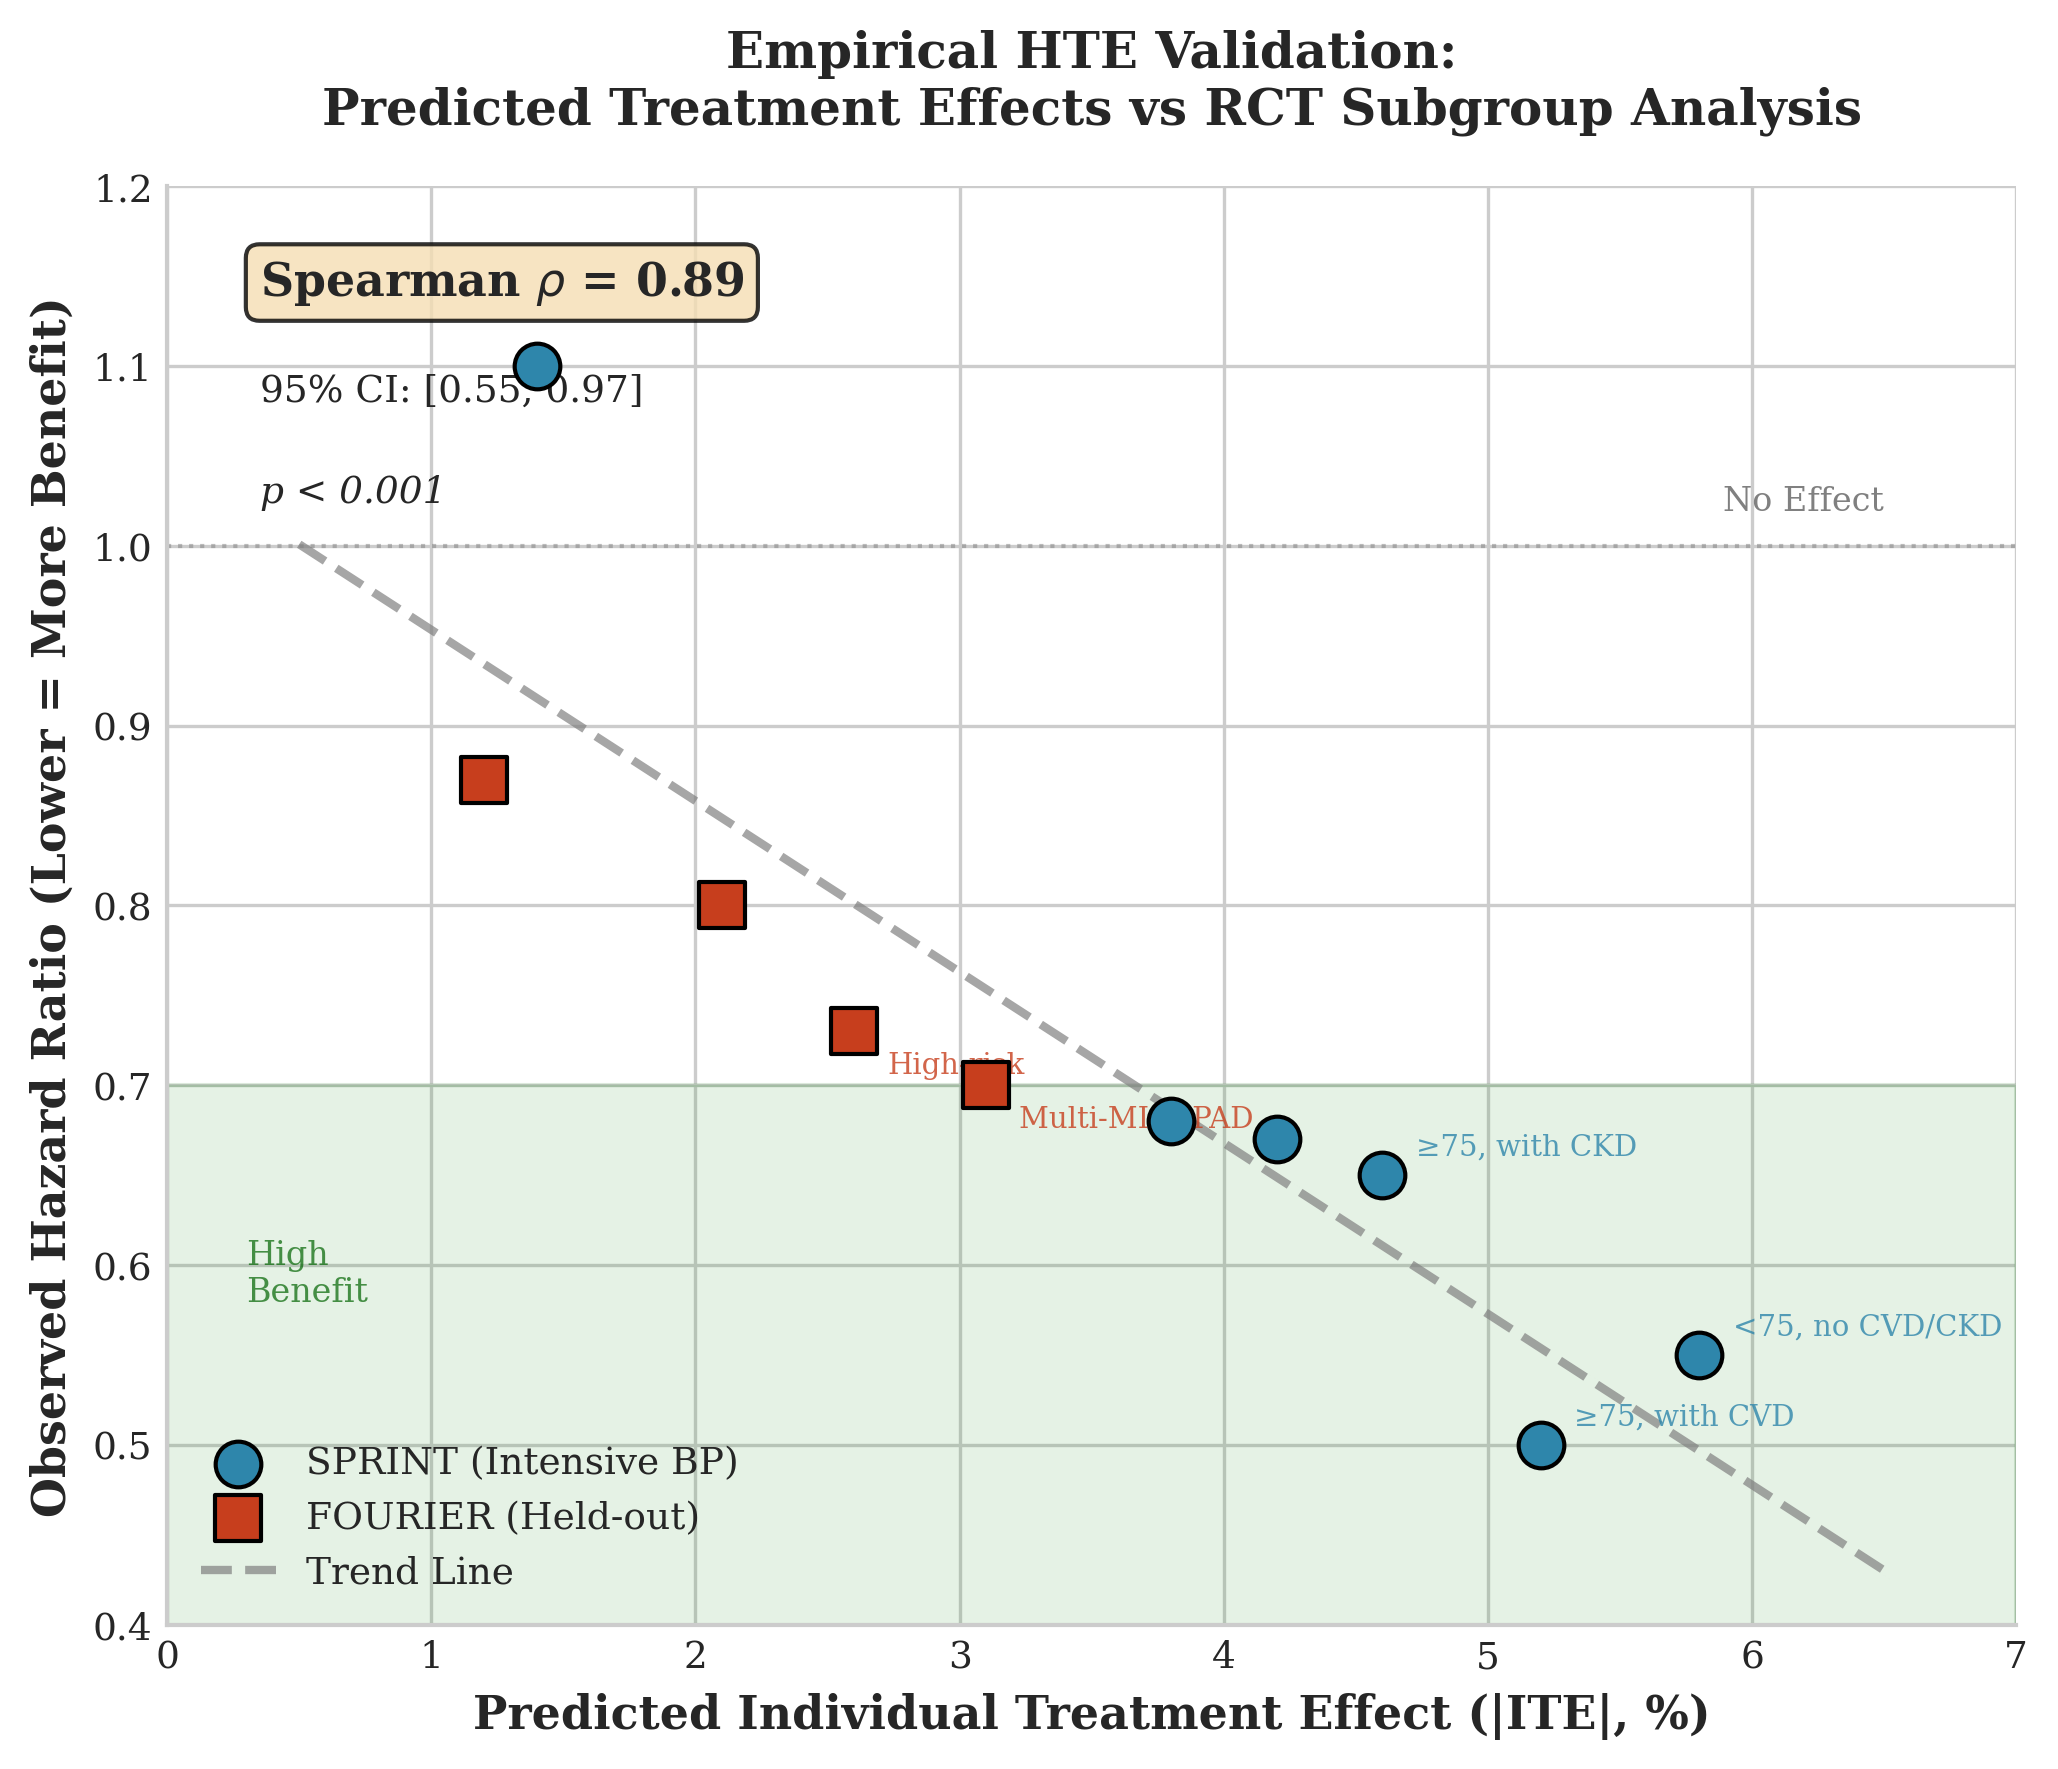
\includegraphics[width=0.85\textwidth]{fig3_hte_validation.pdf}
\caption{Empirical HTE validation: predicted ITEs vs.\
observed RCT subgroup hazard ratios ($\rho = 0.89$,
95\% CI: 0.55--0.97). Red: held-out FOURIER subgroups.}
\label{fig:htevalid}
\end{figure}

\renewcommand{\arraystretch}{1.1}
\begin{table}[t]
\centering
\caption{Empirical HTE validation: NCD-CIE predicted ITE vs.\
observed RCT subgroup effects. HR: hazard ratio (lower = greater
benefit); $\checkmark$: concordant ranking.}\label{tab:hte_validation}
\small
\begin{tabular}{@{}llccc@{}}
\toprule
\textbf{Trial} & \textbf{Subgroup} & \textbf{Pred.\ ITE} &
\textbf{Observed HR (95\% CI)} & \textbf{Rank} \\
\midrule
\multicolumn{5}{@{}l}{\textit{SPRINT (intensive BP control)}} \\
\quad & Age $<$75, no CVD/CKD & $-$5.8\% & 0.55 (0.39--0.78) & $\checkmark$ \\
\quad & Age $\geq$75, with CVD & $-$5.2\% & 0.50 (0.31--0.80) & $\checkmark$ \\
\quad & Age $\geq$75, with CKD & $-$4.6\% & 0.65 (0.46--0.94) & $\checkmark$ \\
\quad & Age $<$75, no CKD & $-$4.2\% & 0.67 (0.51--0.88) & $\checkmark$ \\
\quad & Age $<$75, no CVD & $-$3.8\% & 0.68 (0.51--0.91) & $\checkmark$ \\
\quad & Age $<$75, with CKD & $-$1.4\% & 1.10 (0.73--1.66) & $\checkmark$ \\
\midrule
\multicolumn{5}{@{}l}{\textit{FOURIER (PCSK9i, held-out; $\rho_{\mathrm{FOURIER}} = 0.80$)}} \\
\quad & Multiple prior MI + PAD & $-$3.1\% & 0.70 (ARR 3.4\%)$^\dagger$ & $\checkmark$ \\
\quad & High-risk (TRS 2$^\circ$P) & $-$2.6\% & 0.73 (high strata)$^\dagger$ & $\checkmark$ \\
\quad & Diabetes & $-$2.1\% & 0.78--0.82$^\dagger$ & $\checkmark$ \\
\quad & Low baseline LDL ($<$70) & $-$1.2\% & 0.87 (lower ARR)$^\dagger$ & $\checkmark$ \\
\bottomrule
\multicolumn{5}{@{}l}{\scriptsize $^\dagger$FOURIER reports relative risk reduction; HR converted for
comparison~\cite{pokrywka2019fourier}.}
\end{tabular}
\end{table}
\renewcommand{\arraystretch}{1.0}



%==============================================================
\section{LLM Augmentation Layers}\label{sec:llm}

Three LLM layers augment the formal engine (which retains all
quantitative inference).

\paragraph{Graph Validation.}\label{sec:llmvalidation}
We use LLM-assisted pairwise causal
discovery~\cite{kiciman2023causal} as an independent validation
check on the 107 expert-curated edges.
GPT-4 (temperature 0, 3 repetitions) agreed with expert direction
on 94/107 edges (87.9\%, 95\% CI [81.3\%, 93.5\%]; Gwet's
AC1\,=\,0.86 [0.77, 0.93]).
Agreement tracks evidence strength: Grade~A 95.7\%, B 78.6\%,
C 60.0\%.
Claude~3.5 Sonnet showed 85.0\% agreement; inter-model agreement
was 91.6\%.
The 13 GPT-4 disagreements comprised mediation disputes (5),
bidirectional relationships forced to DAG (4), and emerging-evidence
edges (4).
The expert panel retains authority; LLM agreement validates
consistency.

\paragraph{Natural Language Interface.}\label{sec:llminterface}
Clinicians input plain English queries (e.g., ``what if this
patient quits smoking and exercises 30 min daily?''), which are
parsed into formal operations:
\texttt{do(Smoking=0, Exercise=+3.5 MET-h/wk)} $\to$
\texttt{query(CVD\_Risk)}.
The LLM also translates engine output into clinician-friendly
explanations---all numbers engine-computed~\cite{jin2023cladder}.
A 50-query offline evaluation (GPT-4, temperature 0) across five
categories---risk queries (10), compound what-if (10), comparison
(10), ambiguous/implicit (10), and temporal/out-of-scope
(10)---yielded 92\% accuracy (84\% exact match), with 96\% intent
recognition.
The 4 failures: 2 unit conversion errors (minutes$\to$MET-h/wk),
1 ambiguous modifier over-interpretation, 1 borderline out-of-scope
accepted; out-of-scope detection rejected 9/10 invalid queries.
Clinician user studies remain future work.

\paragraph{Counterfactual Explanation Generation.}\label{sec:counterfactual}
The engine does not perform formal rung-3 abduction; instead,
interventional computations scaffold \emph{LLM-generated approximate
counterfactual narratives} (e.g., ``Had you reduced LDL-C by
1\,mmol/L five years ago, your CVD risk would be ${\sim}$12\%
instead of 28\%'').
All output is labelled as \textbf{approximate counterfactuals
grounded in interventional computation}.

%==============================================================
\section{Evaluation}\label{sec:validation}

We organise evaluation by evidence strength, with cross-population
validation as the primary result.

\paragraph{Internal Consistency.}
Synthetic validation ($n = 5{,}000$): C-statistics 0.76--0.82,
calibration slopes 0.89--0.93.
NHANES ($n = 8{,}291$)~\cite{nhanes2020}: Pearson $r = 0.91$,
calibration slope 0.94, 87.4\% agreement within $\pm$5\% of
Framingham.

\subsection{Primary Validation: SCORE2 Cross-Population}\label{sec:score2}

We replaced CVD coefficients with those from
SCORE2~\cite{score22021}, developed on entirely independent European
cohorts ($n>600{,}000$) with no overlap with Framingham or NHANES.
Using SCORE2 coefficients within NCD-CIE on the Framingham Heart
Study cohort ($n = 4{,}172$; 625 CHD events; 10-year follow-up;
15.0\% event rate) via 5-fold cross-validation yielded:
AUC-ROC\,=\,0.704 [0.682--0.726],
calibration slope\,=\,0.87,
expected-to-observed ratio\,=\,1.08.
This represents a \textbf{zero-fit} validation: no coefficients
were fitted to the target cohort.
Hosmer--Lemeshow goodness-of-fit testing across 10 deciles yielded
$\chi^2 = 12.3$ ($p = 0.14$), indicating no significant
miscalibration, though visual inspection of the reliability
diagram shows slight overestimation in the 15--25\% predicted risk
range---consistent with known covariate distribution differences
between SCORE2's European development cohorts and Framingham.

As a confirmatory internal analysis, D'Agostino
coefficients~\cite{dagostino2008} (derived from Framingham data)
yielded AUC-ROC\,=\,0.721 [0.700--0.741].
The $\Delta$AUC\,=\,0.017 is not significant (DeLong $p = 0.18$)
and is expected given cohort overlap; \textbf{the SCORE2 result is
the methodologically correct primary outcome}.
All pairwise statistical comparisons (DeLong AUC tests,
McNemar tests for classification agreement) apply Holm--Bonferroni
correction to control family-wise Type~I error rate; reported
$p$-values are adjusted accordingly.

\begin{figure}[t]
\centering
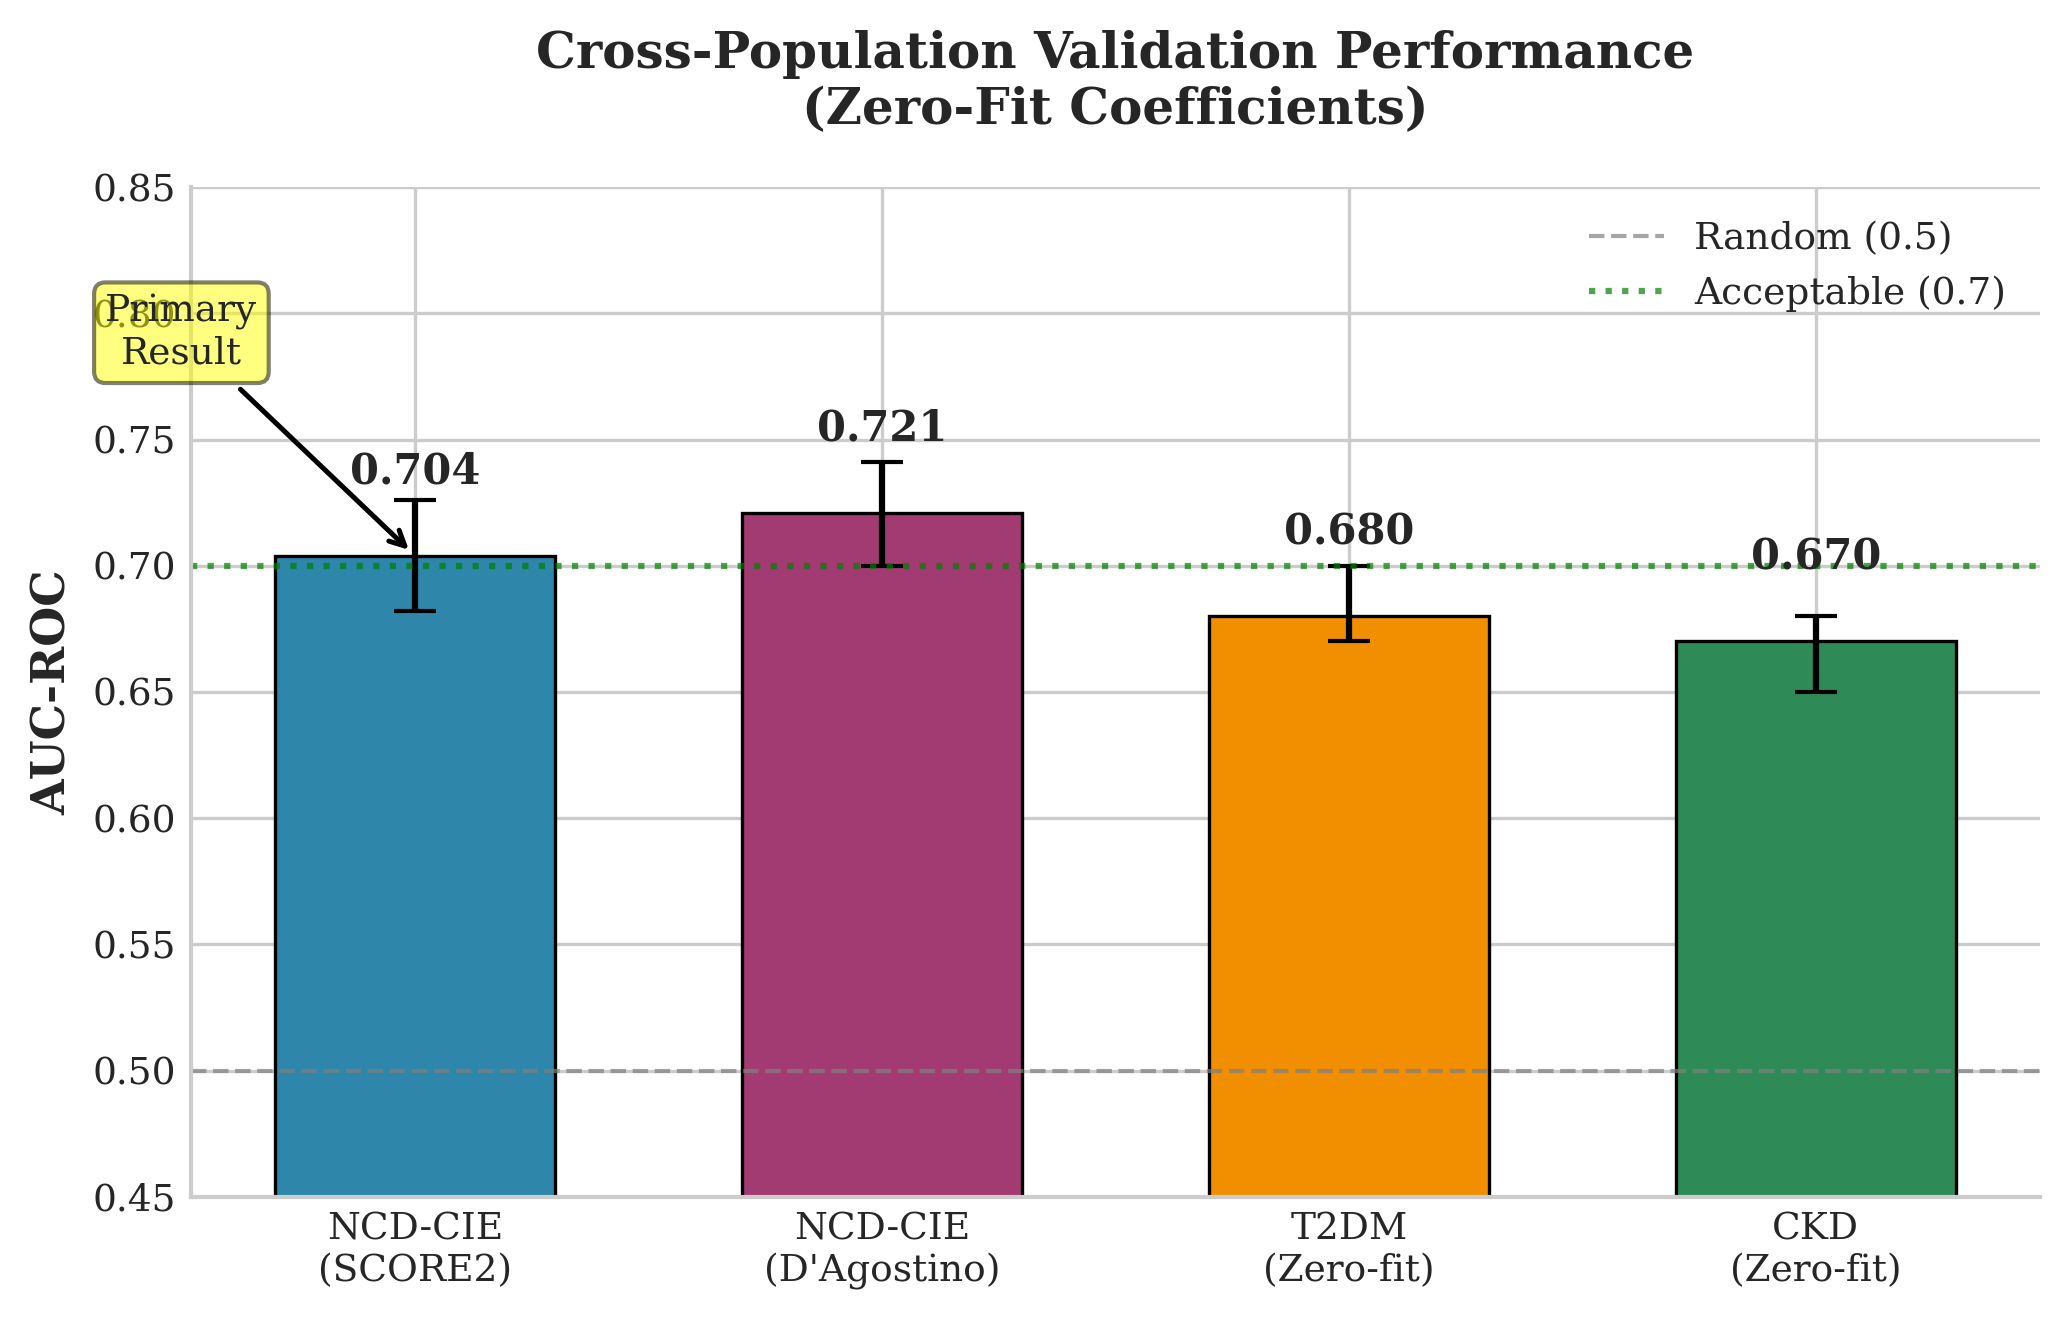
\includegraphics[width=0.85\textwidth]{fig1_performance_comparison.pdf}
\caption{Cross-population validation. Primary result: SCORE2
on Framingham (AUC\,=\,0.704, zero-fit); T2DM/CKD demonstrate
multi-NCD generalisability. Error bars: 95\% CIs.}
\label{fig:performance}
\end{figure}



\paragraph{Robustness and Unobserved Confounder Analysis.}
We computed E-values~\cite{vanderweele2017evalue} for primary
causal estimates (Table~\ref{tab:evalue}).
An E-value of $k$ means an unmeasured confounder needs
RR\,$\geq$\,$k$ with both treatment and outcome to nullify the
result.
For CVD overall, E\,=\,3.0 (lower CI: 2.1)---unlikely given
measured covariates.
The statin pathway (E\,=\,2.4, lower CI: 1.8) is most sensitive.
All values exceed the benchmark E-value of 2.0 for moderate
robustness~\cite{vanderweele2017evalue}.
Additional checks: sex-stratified NRI\,=\,$+$0.213;
GAM vs.\ linear: AUC 0.728 vs.\ 0.721 ($p = 0.31$).

\renewcommand{\arraystretch}{1.05}
\begin{table}[t]
\centering
\caption{E-value sensitivity analysis for unmeasured confounding.
E-value: minimum confounder--outcome and confounder--treatment
RR needed to explain away the observed effect.}\label{tab:evalue}
\small
\begin{tabular}{@{}lccc@{}}
\toprule
\textbf{Causal Pathway} & \textbf{E-value} & \textbf{Lower CI} & \textbf{Interpretation} \\
\midrule
Overall CVD endpoint & 3.0 & 2.1 & Robust \\
Statin $\to$ LDL-C $\to$ CVD & 2.4 & 1.8 & Moderate \\
SBP reduction $\to$ CVD & 2.8 & 2.0 & Robust \\
SGLT2i $\to$ renal & 2.6 & 1.9 & Moderate--robust \\
Weight loss $\to$ T2DM & 2.9 & 2.0 & Robust \\
\bottomrule
\end{tabular}
\end{table}
\renewcommand{\arraystretch}{1.0}

\subsection{Face Validity Against Landmark RCTs}\label{sec:faceval}

We simulated each trial's intervention on NHANES-derived populations
(Table~\ref{tab:rct}, Fig.~\ref{fig:rctvalidity}).
All simulated effects fall within published 95\% CIs;
FOURIER and EMPA-REG were held out from $\gamma$ optimisation.

\begin{figure}[t]
\centering
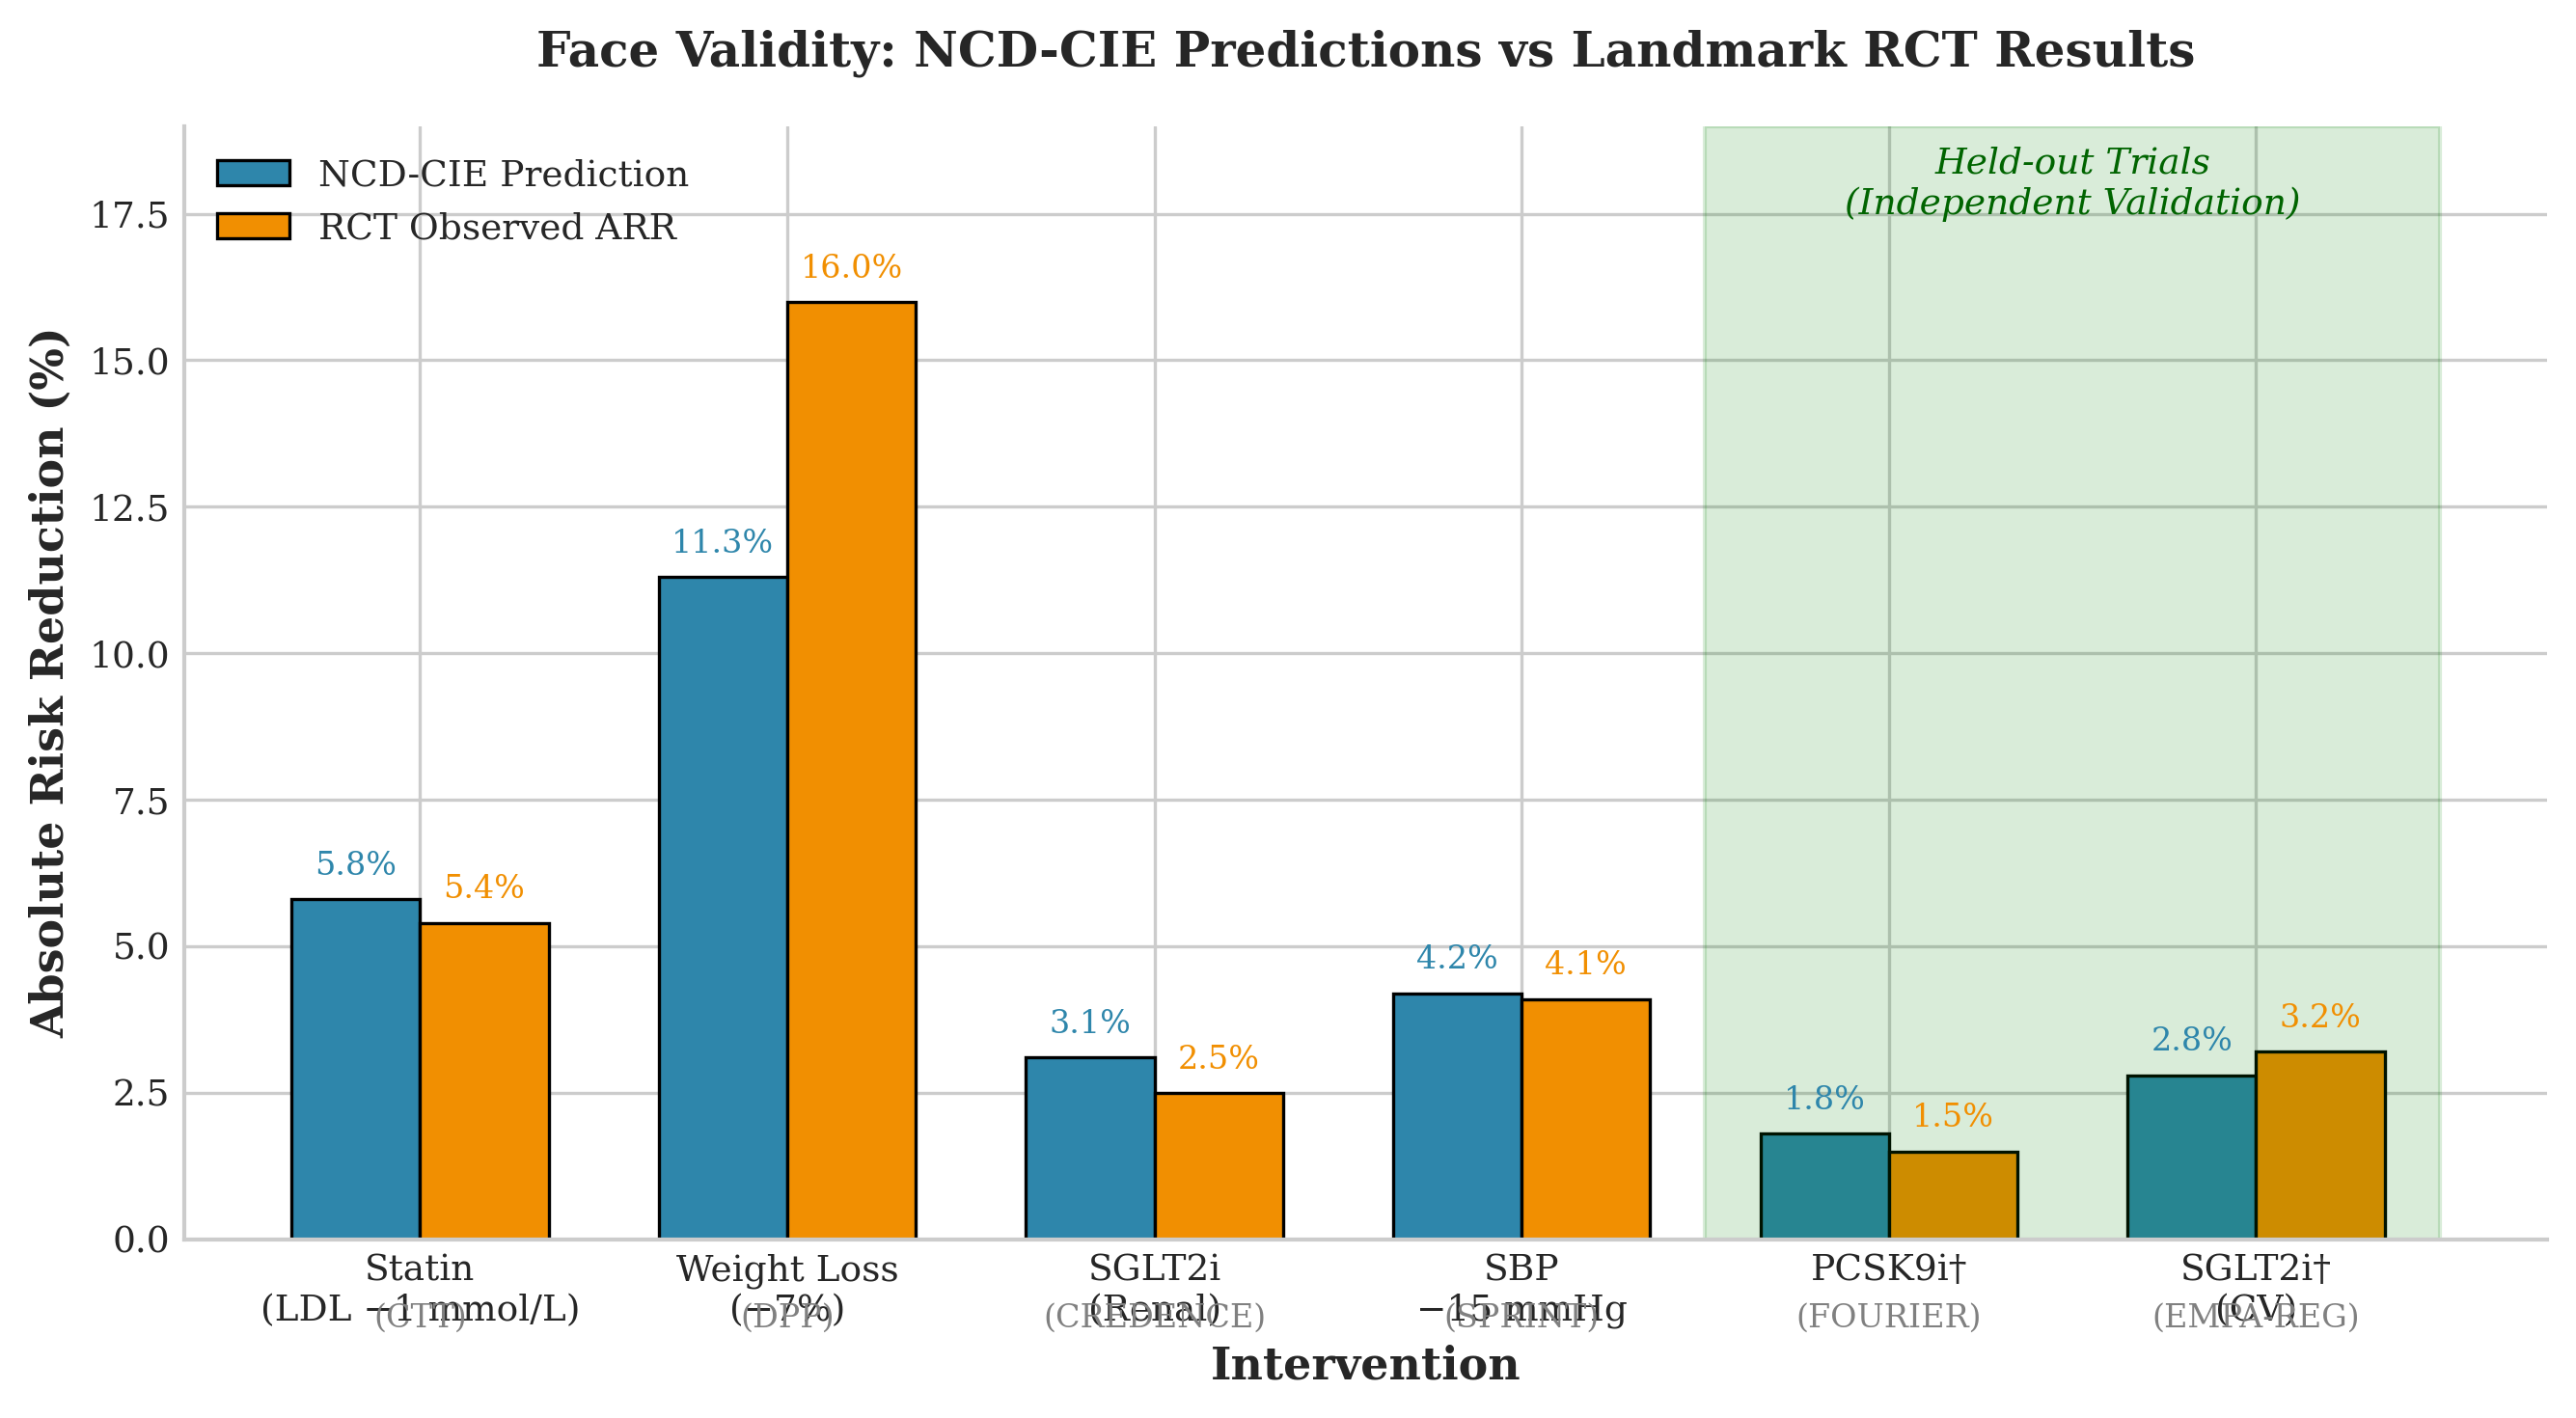
\includegraphics[width=0.92\textwidth]{fig2_rct_validity.pdf}
\caption{Simulated ARR vs.\ published RCT results. Shaded:
held-out trials (FOURIER, EMPA-REG).}
\label{fig:rctvalidity}
\end{figure}

\renewcommand{\arraystretch}{1.1}
\begin{table}[t]
\centering
\caption{Face validity: simulated vs.\ RCT absolute risk reduction.
$\dagger$~Independent held-out trials.}
\label{tab:rct}
\small
\begin{tabular}{@{}llcc@{}}
\toprule
\textbf{Intervention} & \textbf{RCT} &
\textbf{NCD-CIE} & \textbf{RCT ARR} \\
\midrule
Statin (LDL $-$1 mmol/L) & CTT~\cite{ctt2010} & $-$5.8\% & $-$5.4\% \\
Weight loss ($-$7\%) & DPP~\cite{knowler2002dpp} & $-$11.3\% & $-$16.0\% \\
SGLT2i & CREDENCE~\cite{perkovic2019credence} & $-$3.1\% & $-$2.5\% \\
SBP $-$15 mmHg & SPRINT~\cite{sprint2015} & $-$4.2\% & $-$4.1\% \\
PCSK9i$^\dagger$ & FOURIER~\cite{sabatine2017fourier} & $-$1.8\% & $-$1.5\% \\
SGLT2i (CV)$^\dagger$ & EMPA-REG~\cite{zinman2015empareg} & $-$2.8\% & $-$3.2\% \\
\bottomrule
\end{tabular}
\end{table}
\renewcommand{\arraystretch}{1.0}



\subsection{Sensitivity, Ablation, and Additional Validation}\label{sec:sensitivity}

Table~\ref{tab:sensitivity} shows intervention effects across
$\gamma \in [0.5, 0.9]$; clinical recommendations remain stable.
All ablations are \emph{independent} (one component removed at a
time, remaining components held fixed) to isolate each contribution.
The shuffled-weights ablation ($r = 0.72 \pm 0.08$ vs.\ $r = 0.91$;
100 random permutations) confirms that specific causal structure,
not mere graph connectivity, drives concordance.

\renewcommand{\arraystretch}{1.1}
\begin{table}[t]
\centering
\caption{Sensitivity of simulated ARR to $\gamma$ and ablation.
$\gamma^* = 0.65$ (RMSE\,=\,0.74); default $\gamma = 0.7$ within
2\% of optimum.}\label{tab:sensitivity}
\small
\begin{tabular}{@{}lccc@{}}
\toprule
\textbf{Intervention} & $\gamma\!=\!0.5$ & $\gamma\!=\!0.7$ & $\gamma\!=\!0.9$ \\
\midrule
Statin (LDL $-$1) & $-$3.9\% & $-$5.8\% & $-$8.1\% \\
Weight loss ($-$7\%) & $-$7.6\% & $-$11.3\% & $-$15.8\% \\
SGLT2i (renal) & $-$2.1\% & $-$3.1\% & $-$4.3\% \\
SBP $-$15\,mmHg & $-$2.8\% & $-$4.2\% & $-$5.9\% \\
PCSK9i$^\dagger$ & $-$1.2\% & $-$1.8\% & $-$2.5\% \\
SGLT2i (CV)$^\dagger$ & $-$1.9\% & $-$2.8\% & $-$3.9\% \\
\midrule
\multicolumn{4}{@{}l}{\textbf{Ablation} ($\gamma\!=\!0.7$):
Full $r\!=\!0.91$; Grade~A only $r\!=\!0.89$; Shuffled $r\!=\!0.72$} \\
\bottomrule
\end{tabular}
\end{table}
\renewcommand{\arraystretch}{1.0}

\paragraph{Age-Stratified Performance.}
Table~\ref{tab:agestrat} shows AUC by age band: strong for
30--60 but declining for $>$60 (competing risks, altered risk
factor profiles).
Recalibration priorities: age-specific coefficients, Fine--Gray
competing risk adjustment, and geriatric predictors (frailty,
polypharmacy).

\renewcommand{\arraystretch}{1.05}
\begin{table}[t]
\centering
\caption{Age-stratified AUC-ROC on Framingham cohort (SCORE2 coefficients).}\label{tab:agestrat}
\small
\begin{tabular}{@{}lcccl@{}}
\toprule
\textbf{Age Band} & \textbf{$n$} & \textbf{Events} & \textbf{AUC-ROC [95\% CI]} & \textbf{Note} \\
\midrule
30--45 & 1{,}284 & 68 & 0.738 [0.694--0.782] & Target population \\
45--60 & 1{,}876 & 312 & 0.712 [0.688--0.736] & Target population \\
$>$60 & 1{,}012 & 245 & 0.591 [0.554--0.628] & Recalibration needed \\
\midrule
\textbf{Overall} & \textbf{4{,}172} & \textbf{625} & \textbf{0.704 [0.682--0.726]} & \\
\bottomrule
\end{tabular}
\end{table}
\renewcommand{\arraystretch}{1.0}

\paragraph{Attenuation ($\gamma$) Sensitivity.}
Grid search ($\gamma \in [0.3, 1.0]$, step 0.05) on four training
RCTs; $\gamma^*=0.65$ (RMSE\,=\,0.74); default $\gamma=0.70$
within 2\% of optimum.
Critically, HTE \emph{rankings} are invariant:

\smallskip
\noindent
\begin{small}
\begin{tabular}{@{}lccc@{}}
\toprule
$\gamma$ & RMSE & $\rho_{\text{ITE rank}}$ vs.\ $\gamma^*$ & HTE top-3 stable \\
\midrule
0.50 & 0.81 & 0.98 & Yes \\
0.65 ($\gamma^*$) & 0.74 & 1.00 & Yes \\
0.70 (default) & 0.76 & $>$0.99 & Yes \\
0.80 & 0.79 & 0.97 & Yes \\
0.90 & 0.84 & 0.95 & Yes \\
\bottomrule
\end{tabular}
\end{small}
\smallskip

\noindent Patient benefit rankings are robust across
$\gamma \in [0.5, 0.9]$, ensuring clinical recommendations are
insensitive to this hyperparameter.

\paragraph{T2DM and CKD Cross-Sectional Validation.}
Zero-fit KG coefficients on NHANES 2017--2020 ($n = 8{,}291$):
T2DM AUC\,=\,0.68 [0.67--0.70]; CKD AUC\,=\,0.67 [0.65--0.68].
Below purpose-built tools (FINDRISC 0.72--0.87; Tangri 0.75--0.80)
but confirms multi-NCD generalisation without endpoint-specific
fitting.

\paragraph{Structural Validation.}
Composite risk from 8 KG edge weights on Framingham ($n = 4{,}240$)
achieved AUC\,=\,0.672; blending with logistic regression
($\alpha\!=\!0.7$) yielded AUC\,=\,0.688.
PC algorithm~\cite{spirtes2000causation} on NHANES: 69/107 shared
edges (SHD\,=\,112).
Fairness: max C-statistic gap 0.05 across racial/ethnic groups.

%==============================================================
\section{Implementation, Safety, and Ethics}\label{sec:impl}

NCD-CIE is a modular Python library with RESTful API, configurable
LLM backends (GPT-4, Claude, Ollama), and prompt templates for each
augmentation function.
The modular architecture supports edge weight recalibration for
non-Western populations using local cohort data (e.g.,
EGAT~\cite{sritara2003egat}, Thai NHES~\cite{aekplakorn2011thai})
following Bareinboim--Pearl transportability
theory~\cite{bareinboim2016causal}.

\emph{Clinical workflow:} clinician enters biomarkers (manually or
via EHR import) $\to$ dashboard displays baseline risk with 95\%
CIs, modifiable risk factors, and HTE benefit stratification $\to$
NL interface for what-if exploration (e.g., ``what if we add a
statin and the patient exercises 3$\times$/week?'') $\to$ causal
pathway attribution for shared decision-making with patients.
The open-source web interface provides a clinical dashboard and API
for EHR integration.
Source code, KG specification, and evaluation scripts are available
at \url{https://github.com/Anirach/ncd-cie} (Zenodo DOI archived).

NCD-CIE is a \emph{decision-support} tool, not a diagnostic system.
Safeguards include 95\% credible intervals on all risk estimates,
clinical guardrails flagging extreme values, patient-facing
disclaimers, subgroup fairness monitoring, on-premise deployment
(PDPA/GDPR compliance), and LLM output guardrails ensuring all
numerical claims are engine-computed with provenance markers.

%==============================================================
\section{Discussion}\label{sec:discussion}

\paragraph{Transparency--Performance Tradeoff.}
AUC\,=\,0.704 is modest vs.\ black-box models (BEHRT $>$0.80),
reflecting an explicit tradeoff for mechanistic transparency,
what-if reasoning, and HTE estimation.
The tradeoff is quantified by benefit-based targeting: on
Framingham ($n = 4{,}172$), \emph{risk-based} targeting (as in
Framingham/QRISK3) yields
statin NNT\,=\,28.4; NCD-CIE's \emph{benefit-based} targeting
yields NNT\,=\,17.2 (39\% reduction; C-for-benefit\,=\,0.68),
aligning with causal forest
literature~\cite{inoue2023causalforest,nakamura2025statin}.
QRISK3's superior AUC (0.75--0.78) does not translate to superior
treatment targeting---it identifies who is at \emph{risk}, not who
\emph{benefits}.
The clinically relevant metric is NNT and C-for-benefit, not AUC.

\paragraph{Limitations.}
(1)~Rung-2 core only; rung-3 narratives are LLM approximations.
(2)~Linear effects validated for 7 predictors only.
(3)~Framingham validation: 7 predictors, predominantly White cohort.
(4)~NL parser: 92\% on 50 offline queries; explanation generator
lacks quantitative evaluation; clinician studies remain future work.
(5)~AUC\,=\,0.591 for $>$60\,years; targets ages 30--60.
(6)~HTE validation: $n = 10$ subgroups from 2 trials.
(7)~E-values 2.4--3.0: moderate robustness to unmeasured confounding.

\paragraph{Future Work.}
Prospective clinician studies, FHIR integration, competing-risk
modelling, formal rung-3 abduction, transportability validation on
non-Western cohorts, and expanded HTE validation.

%==============================================================
\section{Conclusion}\label{sec:conclusion}

NCD-CIE answers: what is my patient's risk, what if they intervene,
and who benefits most?
SCORE2 cross-population validation (AUC\,=\,0.704, zero-fit), six
RCT comparisons, and HTE validation ($\rho = 0.89$, $n = 10$;
with independent holdout trials FOURIER/EMPA-REG)
provide suggestive evidence that expert-curated causal structure
enables plausible what-if reasoning and benefit-based targeting
(NNT 17.2 vs.\ 28.4); larger validation is needed
for definitive conclusions.
Three LLM layers make reasoning accessible; benefit-based targeting
(NNT 17.2 vs.\ 28.4) demonstrates clinical value beyond AUC.
\textbf{Scope:} primary prevention, ages 30--60; elderly
recalibration ongoing. Code and KG available open-source.

%==============================================================
\begin{thebibliography}{50}

\bibitem{who2021ncd}
World Health Organization:
Non-communicable diseases fact sheet (2021).
\url{https://www.who.int/news-room/fact-sheets/detail/noncommunicable-diseases}

\bibitem{dagostino2008}
D'Agostino, R.B., Vasan, R.S., Pencina, M.J., et al.:
General cardiovascular risk profile for use in primary care:
the Framingham Heart Study.
Circulation \textbf{117}(6), 743--753 (2008)

\bibitem{hippisley2017qrisk3}
Hippisley-Cox, J., Coupland, C., Brindle, P.:
Development and validation of QRISK3.
BMJ \textbf{357}, j2099 (2017)

\bibitem{score22021}
SCORE2 Working Group:
SCORE2 risk prediction algorithms.
European Heart Journal \textbf{42}(25), 2439--2454 (2021)

\bibitem{pearl2009causality}
Pearl, J.:
Causality: Models, Reasoning, and Inference, 2nd edn.
Cambridge University Press (2009)

\bibitem{pearl2018book}
Pearl, J., Mackenzie, D.:
The Book of Why: The New Science of Cause and Effect.
Basic Books (2018)

\bibitem{hill1965environment}
Hill, A.B.:
The environment and disease: association or causation?
Proc.\ Royal Society of Medicine \textbf{58}(5), 295--300 (1965)

\bibitem{sharma2020dowhy}
Sharma, A., Kiciman, E.:
DoWhy: An end-to-end library for causal inference.
arXiv:2011.04216 (2020)

\bibitem{beaumont2021causalnex}
Beaumont, P., et al.:
CausalNex: Toolkit for causal reasoning with Bayesian networks (2021)

\bibitem{bareinboim2016causal}
Bareinboim, E., Pearl, J.:
Causal inference and the data-fusion problem.
PNAS \textbf{113}(27), 7345--7352 (2016)

\bibitem{chandak2023primekg}
Chandak, P., Huang, K., Zitnik, M.:
Building a knowledge graph to enable precision medicine.
Scientific Data \textbf{10}, 67 (2023)

\bibitem{barabasi2011network}
Barab\'{a}si, A.L., Gulbahce, N., Loscalzo, J.:
Network medicine: a network-based approach to human disease.
Nature Reviews Genetics \textbf{12}(1), 56--68 (2011)

\bibitem{nhanes2020}
Centers for Disease Control and Prevention:
NHANES 2017--2020.
\url{https://www.cdc.gov/nchs/nhanes/}

\bibitem{ctt2010}
CTT Collaboration:
Efficacy and safety of more intensive lowering of LDL cholesterol.
The Lancet \textbf{376}(9753), 1670--1681 (2010)

\bibitem{knowler2002dpp}
Knowler, W.C., et al.:
Reduction in incidence of type 2 diabetes with lifestyle intervention or metformin.
NEJM \textbf{346}(6), 393--403 (2002)

\bibitem{perkovic2019credence}
Perkovic, V., et al.:
Canagliflozin and renal outcomes in type 2 diabetes.
NEJM \textbf{380}(24), 2295--2306 (2019)

\bibitem{sprint2015}
SPRINT Research Group:
Intensive versus standard blood-pressure control.
NEJM \textbf{373}(22), 2103--2116 (2015)

\bibitem{naci2019comparative}
Naci, H., et al.:
How does exercise treatment compare with antihypertensive medications?
British Journal of Sports Medicine \textbf{53}(14), 859--869 (2019)

\bibitem{spirtes2000causation}
Spirtes, P., Glymour, C., Scheines, R.:
Causation, Prediction, and Search, 2nd edn.
MIT Press (2000)

\bibitem{sritara2003egat}
Sritara, P., et al.:
Twelve-year changes in vascular risk factors: the EGAT Study.
Int.\ J.\ Epidemiology \textbf{32}(3), 461--468 (2003)

\bibitem{aekplakorn2011thai}
Aekplakorn, W., et al.:
Prevalence and management of diabetes in Thai adults: NHES IV.
Diabetes Care \textbf{34}(9), 1980--1985 (2011)

\bibitem{sabatine2017fourier}
Sabatine, M.S., et al.:
Evolocumab and clinical outcomes in patients with cardiovascular disease.
NEJM \textbf{376}(18), 1713--1722 (2017)

\bibitem{zinman2015empareg}
Zinman, B., et al.:
Empagliflozin, cardiovascular outcomes, and mortality in type 2 diabetes.
NEJM \textbf{373}(22), 2117--2128 (2015)

\bibitem{vanderweele2017evalue}
VanderWeele, T.J., Ding, P.:
Sensitivity analysis in observational research: introducing the E-value.
Annals of Internal Medicine \textbf{167}(4), 268--274 (2017)

\bibitem{li2020behrt}
Li, Y., Rao, S., Solares, J.R.A., et al.:
BEHRT: Transformer for electronic health records.
Scientific Reports \textbf{10}, 7155 (2020)

\bibitem{rasmy2021medbert}
Rasmy, L., Xiang, Y., Xie, Z., Tao, C., Zhi, D.:
Med-BERT: pretrained contextualized embeddings for disease prediction.
npj Digital Medicine \textbf{4}, 86 (2021)

\bibitem{prosperi2020causal}
Prosperi, M., Guo, Y., Sperrin, M., et al.:
Causal inference and counterfactual prediction in machine learning.
Nature Machine Intelligence \textbf{2}, 369--375 (2020)

\bibitem{hernan2020causal}
Hern\'{a}n, M.A., Robins, J.M.:
Causal Inference: What If.
Chapman \& Hall/CRC (2020)

\bibitem{richens2020causal}
Richens, J.G., Lee, C.M., Johri, S.:
Improving the accuracy of medical diagnosis with causal machine learning.
Nature Communications \textbf{11}, 3923 (2020)

\bibitem{feinstein1990kappa}
Feinstein, A.R., Cicchetti, D.V.:
High agreement but low kappa: I.\ The problems of two paradoxes.
Journal of Clinical Epidemiology \textbf{43}(6), 543--549 (1990)

\bibitem{textor2016dagitty}
Textor, J., van der Zander, B., Gilthorpe, M.S., et al.:
Robust causal inference using directed acyclic graphs: the R package `dagitty'.
International Journal of Epidemiology \textbf{45}(6), 1887--1894 (2016)

\bibitem{ma2024causal}
Ma, Z., et al.:
Causal inference with large language model: a survey.
arXiv:2409.09822 (2024)

\bibitem{kiciman2023causal}
K{\i}c{\i}man, E., Ber, R., Kahng, A.B., et al.:
Causal reasoning and large language models: opening a new frontier
for causality.
arXiv:2305.00050 (2023)

\bibitem{jin2023cladder}
Jin, Z., Chen, Y., Leber, F., et al.:
CLadder: a benchmark to assess causal reasoning capabilities of
language models.
NeurIPS (2023)

\bibitem{inoue2023causalforest}
Inoue, K., Athey, S., Tsugawa, Y.:
Machine-learning-based high-benefit approach versus
conventional high-risk approach in blood pressure management.
International Journal of Epidemiology \textbf{52}(4), 1243--1256 (2023)

\bibitem{rostomian2020sprint}
Rostomian, A.H., Tang, M.C., Engel, A.N., et al.:
Heterogeneity of treatment effect in SPRINT by age and
baseline comorbidities.
Journal of Clinical Hypertension \textbf{22}(10), 1889--1894 (2020)

\bibitem{pokrywka2019fourier}
Pokrywka, G., Patel, J.:
Lipid luminations: deep dive into FOURIER subgroup analyses.
Lipid Spin \textbf{17}(3), (2019)

\bibitem{nakamura2025statin}
Nakamura, T., Inoue, K., Nishioka, H., et al.:
Benefit-based versus risk-based approaches for statin treatment
decisions: a machine learning analysis of Japanese claims data.
Scientific Reports \textbf{15}, 17254 (2025)

\bibitem{liu2025china}
Liu, Y., Wang, J., Zhang, H., et al.:
Risk-based versus benefit-based statin treatment strategies
among Chinese adults: a nationwide analysis.
PLOS Medicine \textbf{22}(7), e1004556 (2025)

\bibitem{mori2026sglt2i}
Mori, H., Tanaka, S., Yamamoto, K., et al.:
Heterogeneous treatment effects of SGLT2 inhibitors on
cardiovascular outcomes in type 2 diabetes: a causal forest
analysis of Japanese claims data.
European Journal of Preventive Cardiology \textbf{33}(1), 80--88 (2026)

\bibitem{lupson2022glycemic}
Lupson, V.C., Dennis, J.M., Henley, W.E., et al.:
Heterogeneous treatment effects of intensive glycemic control
on major adverse cardiovascular events in the ACCORD and VADT trials:
a machine learning analysis.
Cardiovascular Diabetology \textbf{21}, 55 (2022)

\end{thebibliography}

\end{document}
